\section{Graphing}

\subsection{Review problems}

\begin{enumerate}
\item Quadrilateral $ABCD$ is positioned in the coordinate plane so that its vertices have coordinates
\begin{equation*}
A = (5, 7);\quad B = (5, 6);\quad C = (3, 1);\quad D = (-4, -5).
\end{equation*}
Points $E, F, G, H$ are the midpoints of segments $\overline{AB}, \overline{BC}, \overline{CD}, \overline{DA}$, respectively.
\begin{enumerate}
\item Find the coordinates of $E$, $F$, $G$, and $H$.
\item Compute the midpoints of segments $\overline{EG}$ and $\overline{FH}$.
\end{enumerate}
To check your work, the two midpoints computed in part (b) should be the same.
\item Maurine needs to get from $(2,3)$ to $(17,11)$.
\begin{enumerate}
\item If they take the shortest path possible, how much distance would they cover?
\item Suppose Maurine gets distracted while pondering the meaning of life and goes from $(2,3)$ to $(6,6)$, then to $(11, 18)$, then to $(17,10)$, and finally to $(17,11)$. What is the minimum distance Maurine can cover which is consistent with this information? 
\end{enumerate}
\item A line passes through the point $(-5,2)$ and has slope $1/2$.
\begin{enumerate}
\item Write down an equation for this line in point-slope form.
\item Find the slope-intercept form and the standard form of the line.
\end{enumerate}
\item A line passes through the points $(-3,4)$ and $(-3,-4)$. Find an equation for this line.
\item A line passes through the points $(-3,3)$ and $(0,-4)$.
\begin{enumerate}
\item Find the slope of the line.
\item For each of the two given points, find the point-slope form of the line using that point.
\item Find the slope-intercept form and the standard form of the line.
\end{enumerate}
As a check of your answers, rearranging either of the point-slope equations from part (b) should give you the same slope-intercept form and standard form.
\item Let $\ell$ be the line with equation $y = -4x - 2$ and let $P = (-4, 2)$. The point $Q$ on line $\ell$ which is closest to $P$ is the point for which $\overline{PQ}\perp\ell$. As such, if $\ell'$ is the line through $P$ perpendicular to line $\ell$, then $Q$ is the intersection of $\ell$ and $\ell'$.
\begin{enumerate}
\item Find the slope of $\ell'$.
\item Find an equation for $\ell'$.
\item Find the coordinates of $Q$.
\end{enumerate}
\item \begin{enumerate}
\item Of the equations
\begin{equation*}
5x + 4y = 35;\quad (x + 4)^2 + (y - 1)^2 = 10;\quad x^2 + xy + y^2 = 49;\quad x - 2y = -7,
\end{equation*}
which one is an equation for the blue line below?
\item Of the equations
\begin{equation*}
5x + 4y = 35;\quad (x + 4)^2 + (y - 1)^2 = 10;\quad x^2 + xy + y^2 = 49;\quad x - 2y = -7,
\end{equation*}
which one is an equation for the red curve below?
\end{enumerate}
\begin{center}
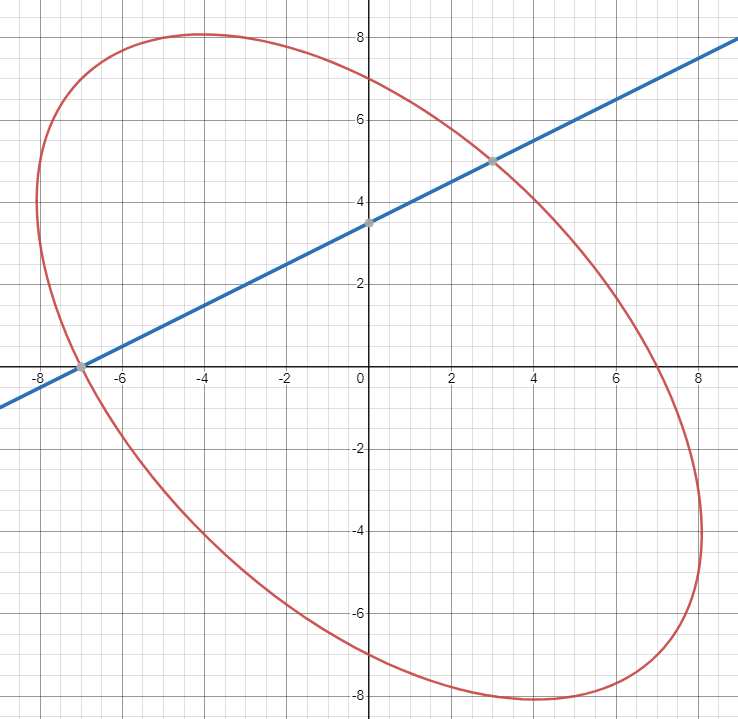
\includegraphics[scale=0.5]{graphing-line-ellipse.png}
\end{center}
\end{enumerate}

\subsection{Challenge problems}

\begin{enumerate}[resume]
\item (Median and centroid) Given any triangle $ABC$, the \emph{medians} are the lines that pass through one vertex and the midpoint of the side opposite that vertex. For example, the $A$-median is the line that passes through $A$ and the midpoint of side $\overline{BC}$. The three medians of a triangle all pass through a single point $G$, called the \emph{centroid} of triangle $ABC$.
\begin{enumerate}
\item Let $A = (0,0)$, $B = (14,0)$, and $C = (5,12)$. Let $D$, $E$, and $F$ be the midpoints of sides $\overline{BC}$, $\overline{CA}$, and $\overline{AB}$, respectively. Find the coordinates of $D$, $E$, and $F$.
\item Find equations for the medians $\overline{AD}$, $\overline{BE}$, and $\overline{CF}$.
\item Find the coordinates of the centroid $G$ of $ABC$. How do they relate to the coordinates of $A$, $B$, and $C$?
\item Compute the ratios $AG/GD$, $BG/GE$, and $CG/GF$.
\end{enumerate}
\item (Altitude and orthocenter) Given any triangle $ABC$, the \emph{altitudes} are the lines that pass through one vertex which are perpendicular to the opposite side. For example, the $A$-altitude is the line that passes through $A$ and is perpendicular to line $\overline{BC}$. The three altitudes of a triangle all pass through a single point $H$, called the \emph{orthocenter} of triangle $ABC$.
\begin{enumerate}
\item Let $A = (0,0)$, $B = (14,0)$, and $C = (5,12)$. Find equations for the altitudes of $ABC$.
\item Find the coordinates of the orthocenter $H$ of $ABC$.
\end{enumerate}
\item Let $A = (1,1)$, $B = (5,2)$, and $C = (-4,3)$. There are three parallelograms in the plane for which $A$, $B$, and $C$ are three of the four vertices. What are the possible coordinates for the fourth vertex?
\end{enumerate}

\newpage
\subsection{Answers}

\begin{enumerate}
\item \begin{enumerate}
\item $E = (5, 13/2)$; $F = (4, 7/2)$; $G = (-1/2, -2)$; $H = (1/2,1)$
\item The midpoint of $\overline{EG}$ is $(9/4, 9/4)$, which is also the midpoint of $\overline{FH}$.
\end{enumerate}
\item \begin{enumerate}
\item $\boxed{17}$
\item $5 + 13 + 10 + 1 = \boxed{29}$
\end{enumerate}
\item \begin{enumerate}
\item $y - 2 = \frac{1}{2}(x + 5)$
\item Slope-intercept form: $y = \frac{1}{2}x + \frac{9}{2}$\par
Standard form: $x - 2y = -9$
\end{enumerate}
\item The line through the two points is the vertical line $\boxed{x = -3}$.
\item \begin{enumerate}
\item $\dfrac{3 - (-4)}{(-3) - 0} = \boxed{-\frac{7}{3}}$
\item Using $(-3,3)$, we get $\boxed{y - 3 = -\frac{7}{3}(x + 3)}$.\par 
Using $(0, -4)$, we get $\boxed{y + 4 = -\frac{7}{3}(x - 0)}$.
\item Slope-intercept form: $\boxed{y = -\frac{7}{3}x - 4}$\par 
Standard form: $\boxed{7x + 3y = -12}$
\end{enumerate}
\item \begin{enumerate}
\item Given a line with slope $m\neq 0$, the slope of any line perpendicular to it is given by $-1/m$. Applying this formula with $m = -4$, the slope of $\ell$, tells us the slope of $\ell'$ must be $\boxed{1/4}$.
\item Using point-slope form, since $\ell'$ passes through $P$, one equation for $\ell'$ is 
\begin{equation*}
\boxed{y - 2 = \frac{1}{4}(x + 4)}.
\end{equation*}
\item Solving the system of equations
\begin{equation*}
y = -4x - 2\qquad\text{and}\qquad y - 2 = \frac{1}{4}(x + 4),
\end{equation*}
we find that $Q = \boxed{(-20/17, 46/17)}$.
\end{enumerate}
\item \begin{enumerate}
\item The blue line passes through $(0, 3.5)$, which only satisfies the equation $\boxed{x - 2y = -7}$.
\item The first and last equation describe lines, so the answer cannot be those. Of the remaining two equations, the point $(7,0)$ on the red curve only satisfies $\boxed{x^2 + xy + y^2 = 49}$.
\end{enumerate}
\item \begin{enumerate}
\item $D = (19/2, 6)$; $E = (5/2, 6)$; $F = (7,0)$
\item $AD$: $y = \frac{12}{19}x$\par
$BE$: $y = -\frac{12}{23}(x - 14)$\par 
$CF$: $y = -6(x - 7)$
\item $G = (19/3, 4)$; the $x$-coordinate of $G$ is the average of the $x$-coordinates of $A$, $B$, and $C$, and a similar statement holds for the $y$-coordinates.
\item $AG/GD = BG/GE = CG/GF = 2$
\end{enumerate}
\item \begin{enumerate}
\item $A$-altitude: $y = \frac{3}{4}x$\par 
$B$-altitude: $y = -\frac{5}{12}(x - 14)$\par 
$C$-altitude: $x = 5$
\item $(5, 15/4)$
\end{enumerate}
\item Each possible fourth vertex $D$ comes from picking two of the three points $A$, $B$, and $C$ to be opposite each other, and then $D$ will be opposite the third point. We will show how to find $D$ in the case that $A$ and $C$ are opposite each other, i.e. the parallelogram is $ABCD$. We will then provide answers for the case that $A$ and $B$ are opposite each other (so the parallelogram is $ACBD$) and the case that $B$ and $C$ are opposite each other (so the parallelogram is $BACD$).\par 
\emph{Solution 1:} If $ABCD$ is a parallelogram, then $\overline{AB}\parallel\overline{CD}$, so $\overline{AB}$ and $\overline{CD}$ have the same slope. The slope of $\overline{AB}$ is $\frac{1 - 2}{1 - 5} = \frac{1}{4}$, so letting $D = (x,y)$,
\begin{equation*}
\frac{y - 3}{x + 4} = \frac{1}{4}.
\end{equation*}
Multiplying both sides by $4(x + 4)$ (i.e. cross multiplying) turns this into the linear equation $4y - 12 = x + 4$. To get another equation, $\overline{BC}\parallel\overline{AD}$, so $\overline{BC}$ and $\overline{AD}$ have the same slope. The slope of $\overline{BC}$ is $\frac{2 - 3}{5 - (-4)} = -\frac{1}{9}$, so 
\begin{equation*}
\frac{y - 1}{x - 1} = -\frac{1}{9}.
\end{equation*}
Cross multiplying gives us $9y - 9 = 1 - x$. We now have two linear equations for the variables $x$ and $y$, and solving the resulting system of equations gives us $(x,y) = \boxed{(-8,2)}$. By similar reasoning, the point which makes $ACBD$ a parallelogram is $D = \boxed{(10,0)}$, and the point which makes $BACD$ a parallelogram is $D = \boxed{(0,4)}$.\par 
\emph{Solution 2:} A geometry theorem states that a quadrilateral $WXYZ$ is a parallelogram if and only if the midpoints of $\overline{WY}$ and $\overline{XZ}$ coincide. Thus for $ABCD$ to be a parallelogram with $D = (x,y)$, we need
\begin{align*}
\text{midpoint of }\overline{AC} &= \text{midpoint of }\overline{BD}, \\
\left(\frac{1 + (-4)}{2}, \frac{1 + 3}{2}\right) &= \left(\frac{5 + x}{2}, \frac{2 + y}{2}\right).
\end{align*}
Matching the first coordinate gives $x = -8$, and matching the second coordinate gives $y = 2$, so $D = \boxed{(-8,2)}$. Similarly, $ACBD$ is a parallelogram when $D = \boxed{(10,0)}$, and $BACD$ is a parallelogram when $D = \boxed{(0,4)}$.
\end{enumerate}